\documentclass{article}

\usepackage[english]{babel}

\usepackage[letterpaper,top=2cm,bottom=2cm,left=3cm,right=3cm,marginparwidth=1.75cm]{geometry}

\usepackage{amsmath}
\usepackage{graphicx}
\usepackage[colorlinks=true, allcolors=blue]{hyperref}
\usepackage{natbib}
\bibliographystyle{alpha}
\usepackage{caption}
\usepackage{float}

\title{Aprendizado de Máquina \\ Trabalho Prático 1}
\author{Luís Felipe Ramos Ferreira \\ 2019022553 \\
    \href{mailto:lframos_ferreira@outlook.com}{\texttt{lframos\_ferreira@outlook.com}}}

\begin{document}
\maketitle

\section{Introdução}

O Trabalho Prático 1 da disciplina de Aprendizado de Máquina teve como tema a criação de uma rede neuronal para classificação de dígitos escritos a mão, mais especificamente o conhecido conjunto de dados \href{https://en.wikipedia.org/wiki/MNIST_database#:~:text=The%20MNIST%20database%20(Modified%20National,the%20field%20of%20machine%20learning.}{\texttt{MNIST}}. Os objetivos do trabalho envolviam analisar como o modelo da rede neuronal iria variar na convergência do erro empírico conforme são modificadas diferentes variáveis de configuração da rede, como a taxa de aprendizado, a quantidade de neurônios na camada oculta e diferentes algoritmos de cálculo de gradiente.

\section{Implementação}

A linguagem escolhida para o desenvolvimento do trabalho foi \href{https://www.python.org/}{\texttt{Python}} (versão 3.10), devida a sua grande variedade de bibliotecas úteis para ciência de dados e aprendizado de máquina. A modelagem da rede neuronal foi feita com o uso da API keras disponibilizada na biblioteca \href{https://www.tensorflow.org/}{\texttt{TensorFlow}}, uma vez que se tratava de uma ferramenta extremamente completa para todos os objetivos do trabalho que permitia grande flexibilidade na modelagem da rede.

Para organizar o ambiente, que englobava várias bibliotecas diferentes, foi utilizado o gerenciador de pacotes \href{https://www.anaconda.com/}{\texttt{Anaconda}}, o que tornou muito mais fácil trabalhar com os pacotes de ciência de dados citados. O projeto final foi salvo em um \href{https://github.com/lframosferreira/MNIST-MLP}{\texttt{repositório}} no GitHub
para fácil versionamento de código e visualização.

\section{Experimentos}

Os experimentos foram realizados sobre uma subparte da base de dados MNIST, disponibilizados no enunciado do trabalho. Essa parte possui um total de 5000 instâncias, que foram divididas em conjunto de treino (90\%) e conjunto de teste (10\%), de modo
que os modelos finais gerados no teste pudessem ser avaliados com o conjunto de treino.

Conforme especificado, foram testados e comparados os resultados da rede neuronal na classificação dos dígitos para diferentes parâmetros de modelagem. Mais especificamente, todas as permutações das seguintes configurações foram utilizadas:

\begin{itemize}
    \item Número de neurônios na camada oculta
        \begin{itemize}
            \item 25
            \item 50
            \item 100
        \end{itemize}
    \item Algoritmo de cálculo de gradiente 
        \begin{itemize}
            \item \textit{Gradient Descent} (O gradiente é calculado após cada época, neste caso, 4500 entradas)
            \item \textit{Stochastic Gradient Descent} (O gradiente é calculado após cada entrada)
            \item \textit{Mini batch} (O gradiente é calculado após um certo número de entradas, neste caso, 10 e 50)
        \end{itemize}
    \item Taxa de aprendizado 
        \begin{itemize}
            \item 0.5
            \item 1.0
            \item 10.0
        \end{itemize}
\end{itemize}

Para fins de analisar também como o número de épocas de treino afeta o modelo, todas as configurações possíveis descritas acima foram utilizadas em modelos que treinaram por 10, 50 e 100 épocas.

O resultado obtido para cada umas das 108 configurações foi armazenado em um arquivo \textit{JSON}, de modo que sua leitura e manipulação fosse facilitada, e assim bibliotecas de análise de dados como \href{https://pandas.pydata.org/}{\texttt{Pandas}} pudessem ser utilizadas para interpretar
como se comportou cada parametrização do modelo durante o treino.

\section{Análise dos resultados de teste}

De maneira geral, os dados gerados deixaram muito claro quais as configurações que permitiam uma boa e uma má performance do modelo. As duas tabelas a seguir mostram os parâmetros das 10 configurações que obtiveram o menor valor de acurácia no conjunto de treino, assim como as 10 configurações com o maior valor de acurácia.

\begin{table}[H]
    \centering
        \captionsetup{labelformat=empty} 
        \caption{10 piores desempenhos}
        \begin{tabular}{| c c c c c |}
        \hline
        Épocas & Tamanho da camada oculta & Tamanho do lote & Taxa de aprendizado & Acurácia \\
        \hline
            100 &  25 &    1 & 10.0 & 0.098 \\
            100 &  50 &    1 & 10.0 & 0.098 \\
            100 & 100 &    1 & 10.0 & 0.098 \\
            10 &  50 &    1 & 10.0 & 0.108 \\
            10 &  25 &    1 & 10.0 & 0.110 \\
            50 &  50 &    1 & 10.0 & 0.120 \\
            50 &  25 &    1 & 10.0 & 0.128 \\
            50 & 100 &    1 & 10.0 & 0.170 \\
            10 &  50 & 4500 & 10.0 & 0.176 \\
            10 & 100 &    1 & 10.0 & 0.182 \\
        \hline
        \end{tabular}
\end{table}

\begin{table}[H]
    \centering
        \captionsetup{labelformat=empty} 
        \caption{10 melhores desempenhos}
        \begin{tabular}{| c c c c c |}
        \hline
        Épocas & Tamanho da camada oculta & Tamanho do lote & Taxa de aprendizado & Acurácia \\
        \hline
            50 & 100 & 10 & 1.0 & 0.946 \\
            50 & 100 & 10 & 0.5 & 0.944 \\
            50 & 100 & 50 & 1.0 & 0.942 \\
            100 & 100 & 10 & 0.5 & 0.942 \\
            10 & 100 & 10 & 1.0 & 0.940 \\
            100 & 100 & 10 & 1.0 & 0.940 \\
            100 & 100 & 50 & 1.0 & 0.940 \\
            10 &  50 & 10 & 0.5 & 0.938 \\
            50 &  50 & 10 & 0.5 & 0.938 \\
            10 & 100 & 50 & 1.0 & 0.936 \\
        \hline
        \end{tabular}
\end{table}

Em primeiro lugar, evidencia-se o fato de que todos os 10 piores valores de acurácia obtidos nos dados de treino ocorreram em modelos com uma taxa de aprendizado igual a 10. Isso indica que uma taxa de aprendizado alta não é uma boa opção para o treino de uma rede neuronal, devido ao fato de que uma alta taxa leva a uma grande quantidade de oscilações durante o treino, gerando alta divergência do erro empírico e, consequentemente, um modelo de baixíssima performance.
Outro fato relevante a se notar é o tamanho dos lotes que geraram os piores resultados. Dentre os 10 piores modelos criados, 9 utilizavam ou o algoritmo \textit{Stochastic Gradient Descent} (tamanho de lote igual a 1). Isso, no entanto, não quer dizer que o uso dessa abordagem seja ruim. O \textit{SGD} é um algoritmo que pode sim gerar bons resultados e ter uma boa performance. O detalhe principal que o levou a aparecer tantas vezes no topo dos piores modelos é a taxa de aprendizado alta, como citada anteriormente. Como a cada entrada os pesos da rede serão alterados, a alta taxa de aprendizado torna ainda mais grave a divergência do erro empírico e causa ainda mais confusão.
Por outro lado, os 10 modelos com os melhores desempenhos em acurácia demonstram que uma taxa de aprendizado equilibrada é um importante fator para um bom resultado. Todos os modelos na tabela contêm taxas de 0.5 ou 1.0. Pode-se notar também que prevalecem entre os melhores modelos tamanhos de lote igual a 10 ou 50, ou seja, o uso do algoritmo \textit{Mini batch} se mostrou o mais performático na construção da rede neuronal. Isso é esperado, dado que a intuição do algoritmo de gradiente \textit{Mini batch} é justamente evitar valores extremos para atualização dos pesos da rede, o que aumenta o poder de generalização da rede.
Por fim, nota-se que 8 entre os 10 modelos com melhor resultado possuem 100 neurônios na camada oculta. Tal fato confirma as hipóteses de que, com mais neurônios, o modelo irá aprender a identificar mais padrões e terá mais poder de generalização. No entanto, deve-se ter cuidado com esse parâmetro da rede, uma vez que números muito altos de neurônios nas camadas ocultas podem gerar problemas relacionados a alta variãncia do modelo gerado.
Em resumo, nota-se que as configurações da rede impactam diretamente em sua performance, e esses parâmetros devem ser estimados com cuidado e suas escolhas feitas considerando cada detalhe necessário para ter um modelo capaz de generalizar bem os dados ao final do treinamento.

\section{Trade-off entre número de unidades da camada oculta e algoritmo de cálculo de gradiente}

Nos gráficos abaixo, podemos ver a variação da acurácia do modelo nos dados de teste em função da variação do número de unidades na camada oculta, para cada um dos algoritmo de cálculo de gradiente propostos.

Ao analisar os diferentes desempenhos da rede neuronal de acordo com a variação entre o número de unidades da camada oculta e o algoritmo de gradiente utilizado, podemos inferir diretamente que o aumento do número de neurônios
causa um impacto positivo no desempenho da maioria dos modelos. Tal inferência faz sentido, uma vez que com uma rede com mais neurônios, mais informações podem ser extraídas e dessa maneira de melhor forma o modelo poderá generalizar sobre
dados ainda não vistos. No entanto, fica claro que um abuso desse hiperparâmetro é algo que pode levar a \textit{overfitting}. Isso fica evidente na análise do algoritmo \textit{Stochastic Gradient Descent}. Como, neste cenário, os pesos da rede são atualizados a cada dado de treino visto, o número alto de neurônios na camada oculta piorou os resultados, muito provavelmente devido
a um problema de variância.

Um fato importante de ser notado é que para a taxa de aprendizado 10.0, que é extremamente alta, o modelo se comporta de forma muito caótica, portanto a análise de seu desempenho conforme a variação do número de neurônios na
camada oculta é prejudicado. No entanto, fica evidente que os modelos que utilizam essa taxa são os piores gerados.

\begin{figure}[H]
    \centering
    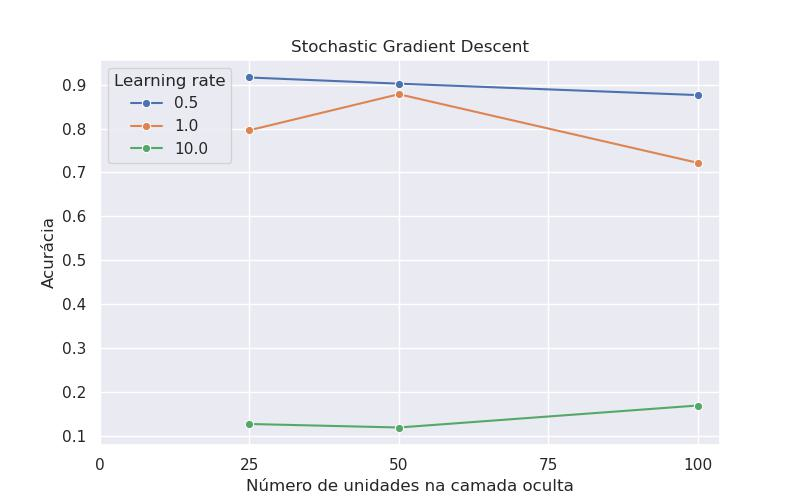
\includegraphics[width=0.8\textwidth]{images/tradeoff/SGD.jpg}
    \caption{Acurácia por número de neurônios para o algoritmo \textit{Stochastic Gradient Descent}}
\end{figure}

\begin{figure}[H]
    \centering
    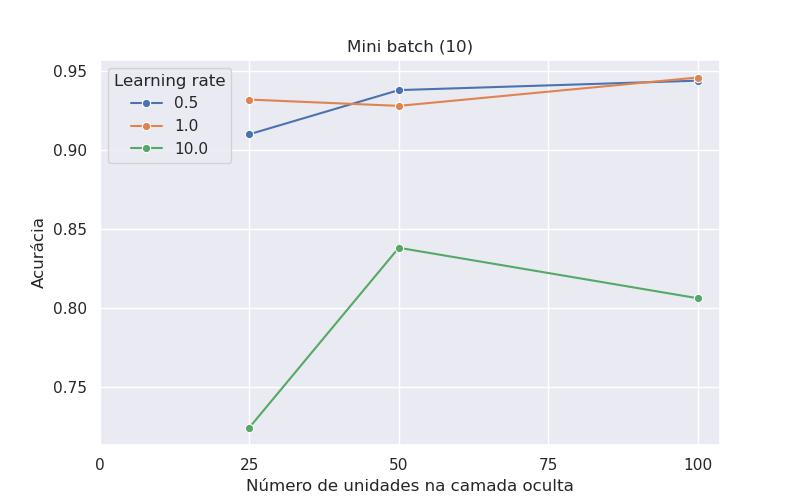
\includegraphics[width=0.8\textwidth]{images/tradeoff/MB10.jpg}
    \caption{Acurácia por número de neurônios para o algoritmo \textit{Mini batch} (10)}
\end{figure}

\begin{figure}[H]
    \centering
    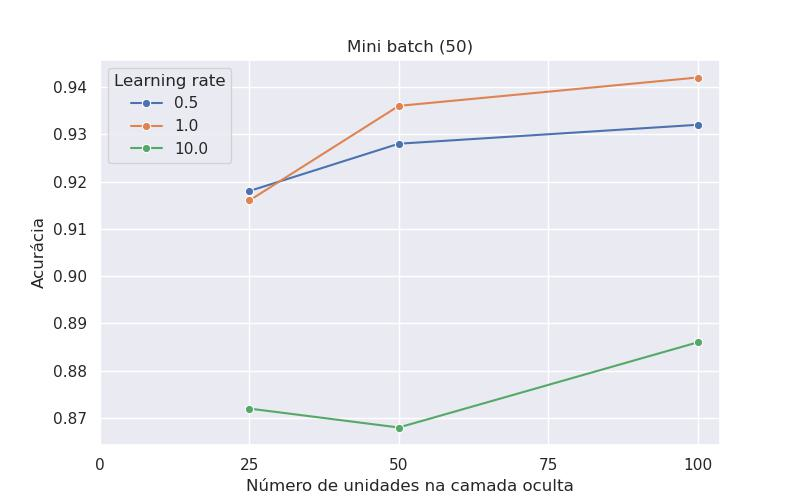
\includegraphics[width=0.8\textwidth]{images/tradeoff/MB50.jpg}
    \caption{Acurácia por número de neurônios para o algoritmo \textit{Mini batch} (50)}
\end{figure}

\begin{figure}[H]
    \centering
    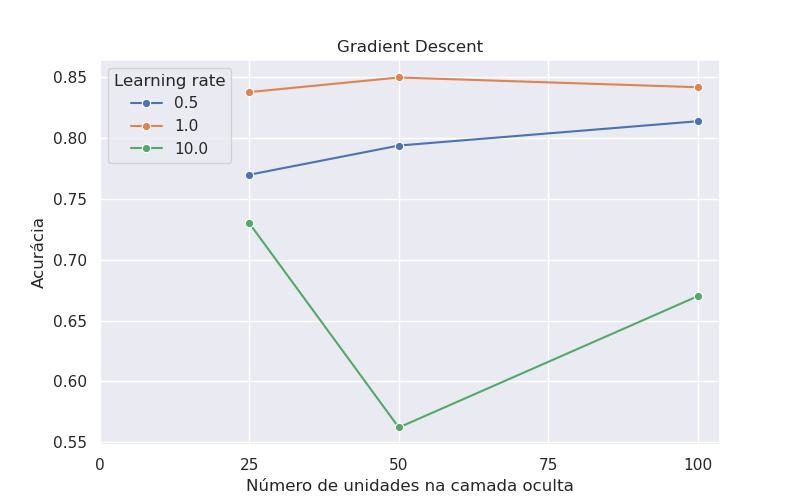
\includegraphics[width=0.8\textwidth]{images/tradeoff/GD.jpg}
    \caption{Acurácia por número de neurônios para o algoritmo \textit{Gradient Descent}}
\end{figure}


\section{Convergência do erro empírico}

Durante o treinamento das redes neuronais propostas, o histórico do erro empírico pode ser armazenado para análise de sua convergência, considerando cada configuração de rede proposta. Para fins de simplificação, serão mostrados
aqui os gráficos de convergência de modelos conforme variação de apenas um hiperparâmetro, enquanto os outros serão escolhidos de forma empírica.

Inicialmente, como discutido em seções anteriores, os modelos que tiveram os melhores resultados de acurácia na fase de teste tinham, de modo geral, 100 neurônios na camada oculta, uma taxa de aprendizado de 0.5 ou 1.0, e utilizavam o algoritmo \textit{Mini batch}.
Tendo essas informações, os seguintes três gráficos foram gerados, em que, baseado nessas constatações, valores fixos para os dois hiperparâmetros não variáveis puderam ser escolhidos.

\begin{figure}[H]
{\centering
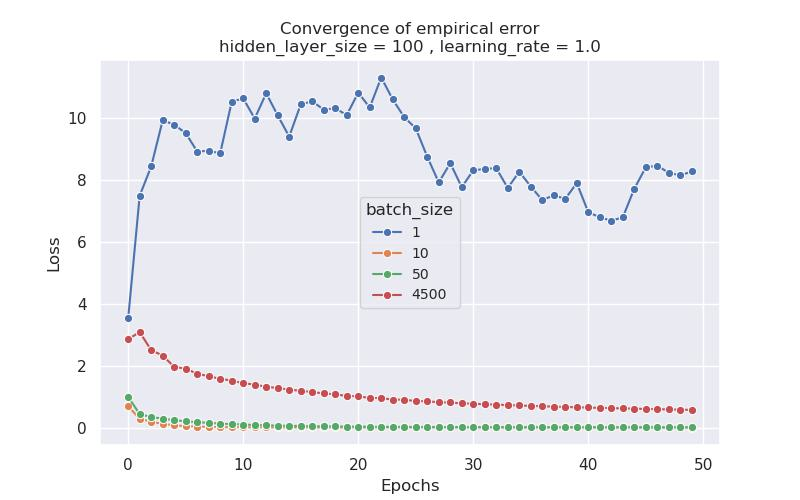
\includegraphics[width=0.8\textwidth]{images/empirical_error/batch_size_not_fixed.jpg}
\caption{Convergência do erro empírico com tamanho do lote (Algoritmo de cálculo de gradiente) variável}}
\end{figure}

Neste primeiro gráfico, podemos ver imediatamente que o algoritmo \textit{Stochastic Gradient Descent} (tamanho do lote igual a 1) foi o que pior performou na convergência do erro empírico
para esta configuração. O seu erro empírivo, inclusive, teve diversas flutuações e sequer pareceu ter algum tipo de convergência que faça sentido. Isso se deve ao fato de que na sua definição, os pesos
da rede são alterados a cada dado de treino, portanto o algoritmo não conseguiu encontrar uma função que generalizasse bem o conjunto de dados
desejado, causando flutuações. Com mais épocas, é possível que o modelo de \textit{SGD} tivesse um melhor desempenho. 

Em relação aos outros algoritmos, nota-se que todos convergiram para erros empíricos bem baixos, com os melhores sendo os que utilizaram o algoritmo \textit{Mini batch} (tamanhos de lote 10 e 50), uma vez
essa configuração permite uma atualização dos pesos em momentos equilibrados, propiciando um melhor ambeinte para convergência do erro empírico.

\begin{figure}[H]
{\centering
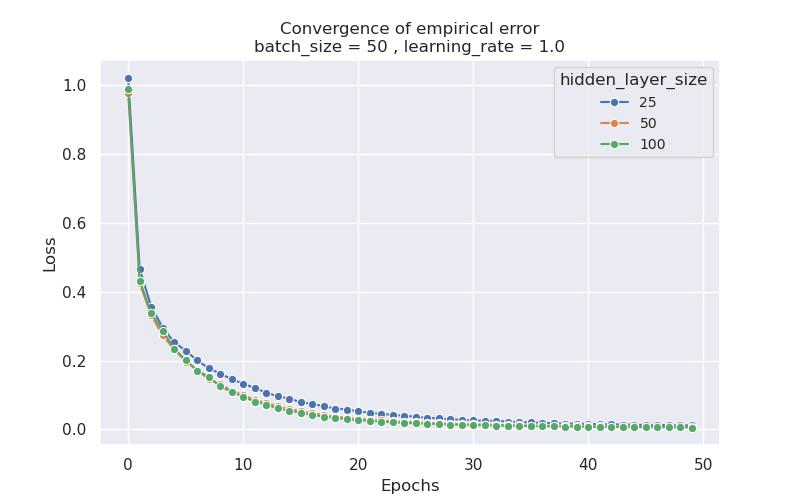
\includegraphics[width=0.8\textwidth]{images/empirical_error/hidden_layer_size_not_fixed.jpg}
\caption{Convergência do erro empírico com tamanho da rede oculta variável}}
\end{figure}

Nesta configuração, nota-se todos os modelos convergiram para valores baixos de erro empírico, com a rede com 100 neurônios na camada oculta convergindo
mais rapidamente e para valores menores. De modo geral, como era de se esperar, aumentar o número de neurônios, para esta configuração, melhora a performance.

\begin{figure}[H]
{\centering
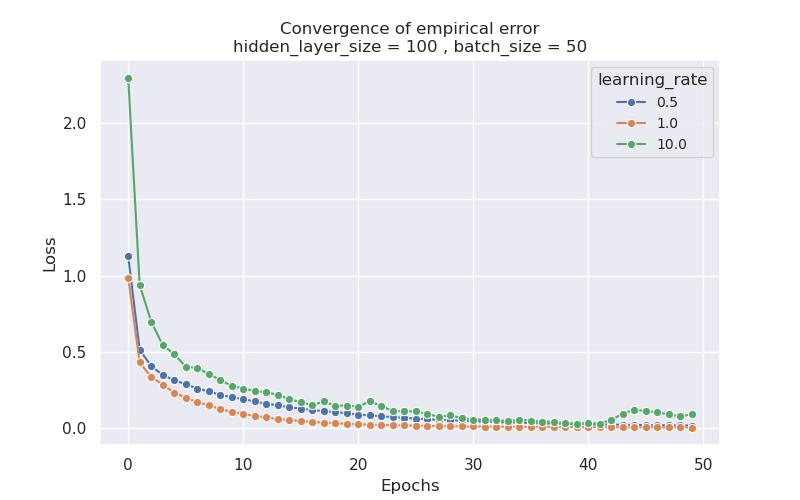
\includegraphics[width=0.8\textwidth]{images/empirical_error/learning_rate_not_fixed.jpg}
\caption{Convergência do erro empírico com taxa de aprendizado variável}}
\end{figure}

Por fim, no gráfico acima, podemos ver que para as configurações escolhidas, o modelo converge para valores baixos de erro empírico conforme o passar das épocas.
Fica claro, conforme também foi discutido anteriormente, que a taxa de aprendizado 10.0 é a pior dentre as três, já que converge para o valor mais alto de erro. Também
como já discutido, isso ocorre pois uma alta taxa de aprendizado gera altas oscilações no treinamento, o que causa um alto nível de divergências nessa etapa.

Em relação aos piores modelos gerados, foi discutido como em todos a taxa de aprendizado igual a 10.0 estava presente, e em 9 dos 10 o algoritmo utilizado foi o \textit{Stochastic Gradient Descent}.
Dessa forma, optou-se por gerar o gráfico referente a uma configuração de rede com estes valores, e o tamanho da rede oculta variável.

\begin{figure}[H]
    \centering
    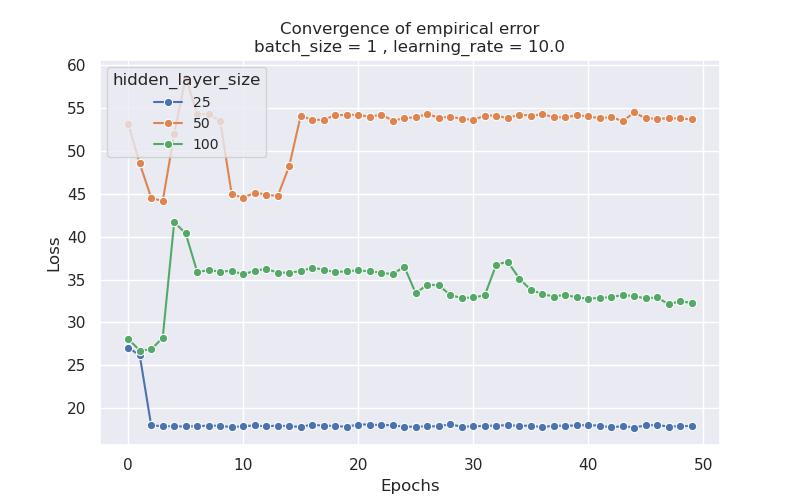
\includegraphics[width=0.8\textwidth]{images/empirical_error/hidden_layer_size_not_fixed_bad.jpg}
    \caption{Convergência do erro empírico com tamanho da rede oculta variável - Piores valores}
\end{figure}

A primeira coisa que se nota ao avaliar esse gráfico é como todos os erros possuem um alto grau de oscilação/divergência. Como era de se
esperar, já que se tratam de modelos com altíssimas taxas de aprendizado e que utilizam o algoritmo \textit{SGD}. Vê-se também
que em todos eles o erro empírico final foi muito alto, com o modelo com 25 neurônios na camada oculta sendo o que convergiu
para o menor deles. Isso se deve ao fato de que, com a alta taxa de aprendizado e uma atualização constante dos pesos, uma rede
com menos neurônios, isto é, mais simples, irá sofrer menos com oscilações.

\section{Conclusão}

conclusão

\end{document}
